\label{ch:2}
%\section{Classical methods for socially complaint navigation}

%\subsection*{Outline structure of the chapter}
%\begin{enumerate}
%    \item Describe the problem of navigation.
%    \item Describe the problem of social navigation and what how is it different from the problem of classical navigation.
%
%    \item What are the factors that make this problem hard to pin and thus hard to solve? Include works from the paper "Influence of proxemic behaviors in human-robot interaction. (Takayama et al)
%    \item Set of works done before and how they try to approach the problem.
%\end{enumerate}
%
%\subsection*{Papers to inculde}
%    \begin{enumerate}
%        \item Social forces model and its family (Reif and wang, Helbing and Molnar).
%        \item Qualitative trajectory calculus
%        \item A framework towards a socially aware mobile robot motion in a human ventured dynamic environment. - Pandey et al
%        \item Dynamic window approach for reactive collision avoidance.
%        \item Human aware mobile robot motion planner - Sisbot
%        \item Trajectory planning for robots in dynamic human environments. Svenstrup
%    \end{enumerate}
%

In this chapter, we go through some of the classical approaches from the existing literature that address the problem of socially-compliant navigation. We will start by briefly describing the method and its strengths, followed by their limitations and the subsequent body of research that improves on it.
%\subsubsection*{Khatib et al}
\par
One of the earliest path planners include A-star algorithm \cite{hart1968} that uses a graph-based heuristic search to determine the path with the least cost between two points. More recent work on controllers for autonomous navigation is based on artificial potential fields \cite{khatib_1986}. The main idea behind the method is that an agent moving through a scene is analogous to a particle moving through a force-field, where the goal exerts an attractive force while the obstacle surfaces negative forces. The resultant force, which is inversely proportional to the distance between these external entities, then guides the agent towards the goal while avoiding incoming obstacles as shown in \autoref{fig:artificial_pf}. The resulting controller, with proper hyper-parameters, does a fairly good job of navigating a scene checking all the boxes of a good navigating agent: it reaches the goal location avoiding obstacles along the way. There are many drawbacks to this method. The most notable being getting stuck in local minima, which were addressed by more sophisticated methods like probabilistic road-map based approaches \cite{Lavalle98rrt}. \\
%\subsubsection*{Helbing and Molnar: Social Forces}
\begin{figure}
	\centering
	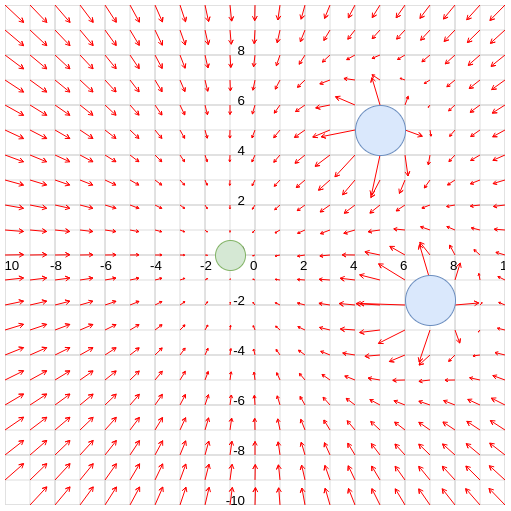
\includegraphics[width=\linewidth]{figures/vector_field_pf.png}
	\caption{Graphical representation of an artificial potential field. The force field guiding any agent  towards the goal at (-1, 0) (green circle) is disrupted by the repulsive forces of the obstacles located at (5,5) and (7, -2))}
	\label{fig:artificial_pf}
\end{figure}
Building on artificial potential fields, Helbing and Molnar introduce a pedestrian model that follows principles similar to that of the artificial potential fields and encapsulates a richer set of information to imbibe `social' behavior in the agent's movement \cite{helbing_social_1998}. Rather than representing the force applied to an agent as the sum of the forces from external factors (obstacles and goal(s)), they model the pedestrian behavior as a combination of a set of internal motivations.\\
%\thcomment{Here "they refers to the work of Helbing and Molnar. Should I change the wording?}

The formulation is given by:
\\
%\thcomment{\cite{helbing_social_1998} in their paper had a bunch of equations describing the different forces acting on the agent, the sum of which is given by the equation \autoref{eq:helbing_final_eq}. I get it. Here, writing 'final' is out of context.}
\begin{align}
\label{eq:helbing_final_eq}
\frac{d\vec{w_{\alpha}}}{dt}:=\vec{F_{\alpha}}(t)+fluctuations
\end{align}
where, $\vec{w_{\alpha}}$ is the preferred velocity of pedestrian $\alpha$ and $\vec{F_{\alpha}}$ is the combined effect of all the forces acting on pedestrian $\alpha$. $\vec{F_{\alpha}}$ is further expanded as:\\
\begin{multline}
\label{eq:lebing_molnar_social_forces}
\vec{F_{\alpha}}(t):=
\vec{F_{\alpha}^{0}}(\vec{v_{\alpha}}, v_{\alpha}^{0}\vec{e_{\alpha}})+\sum_{\beta}\vec{F_{\alpha, \beta}}(\vec{e_{\alpha}}, \vec{r_{\alpha}} - \vec{r_{\beta}})
+\\\sum_{B}\vec{F_{\alpha B}}(\vec{e_{\alpha}}, \vec{r_{\alpha}} - \vec{r_{B}^{\alpha}}) + \sum_{i}\vec{F_{\alpha i}}(\vec{e_{\alpha}}, \vec{r_{\alpha}}-\vec{r_i},t)
\end{multline}
where, $\vec{r_{\alpha}}$,  $\vec{v_{\alpha}}$,  $\vec{v^{0}_{\alpha}}$ and $\vec{e_{\alpha}}$  are the current location, velocity, desired speed and desired direction of pedestrian $\alpha$. $\vec{r^{\alpha}_{B}}$ is the smallest distance between pedestrian $\alpha$ and an obstacle $B$, and, $\vec{r_i}$ is the position of any object, other than the goal, that can temporarily attract a pedestrian. \\
Each of the terms being added up in \autoref{eq:lebing_molnar_social_forces} is a mathematical formulation of an internal motivation.
$\vec{F_{\alpha}^{0}}$ is the force guiding the agent towards the goal, $\vec{F_{\alpha\beta}}$ and  $\vec{F_{\alpha B}}$ denotes the repulsive forces from other pedestrians and obstacles respectively.
$\vec{F_{\alpha i}}$  sums up the attractive forces other than the goal, that might attract a pedestrian like a street artist or a window of a shop.
\par
Careful observation and interpretation of human behavior and engineering rules that resemble them lead to the creation of a controller that provides a social flavor to the previously socially-indifferent controller obtained from artificial potential fields. Formulations of this nature are highly dependent on the different cases being considered and assumptions being made in the creation of the model.
%\textcolor{red}{A lot of careful engineering has been put into creating this 'formulae' that dictate/emulate the naturalness of human-movement while negotiating crowded space in an artificial agent/robot. 
%Formulations of this nature are highly dependent on the different cases being considered and assumptions being made in the creation of the model.}\\

%\subsubsection*{Sisbot et al}
In more recent work \cite{sisbot_human_2007}, Sisbot et al. take a similar approach, where they generate and make use of three different cost maps, $Cost_{safety}$, $Cost_{visibility}$ and $Cost_{hidden zone}$ each focusing on a separate attribute.
The $Cost_{safety}$ keeps track of how safe a location in the grid is based on the structure and kinematics of the human and his/her state, where the state includes information like the posture (sitting or standing), configuration and parameters.
$Cost_{visbility}$ is designed to penalize the robot if it is positioned outside the field-of-view of nearby pedestrians. 
The rationale being, the effort a human has to make to keep the robot in his/her vision is directly proportional to the discomfort caused by the robot with its movements. For example, regions behind a pedestrian is associated with a greater penalty as compared to regions in front.
And lastly, $Cost_{hidden zone}$ takes into account the amount of time when the robot remains hidden behind any obstacle and the penalty associated with it. 
The authors also provide two nuanced ways of merging the cost terms. One where the $Cost_{merged}$ is the weighted sum of two
\begin{align}
Cost_{merged}(x,y) = w_{1}Cost_{safety}(x,y) + w_{2}Cost_{visibility}(x,y)
\end{align}
and 
\begin{align}
Cost_{merged}(x,y) = max(Cost_{safety}(x,y), Cost_{visibility}(x,y))
\end{align}

The final cost function factoring in the $Cost_{hidden zone}$ is
\begin{align}
Cost_{final}(x,y) \leftarrow w_{3} Cost_{hidden zone}(x,y)
\end{align}
when, $x$ and $y$ are in the field of view of a human, but is obstructed by the presence of the robot and 
\begin{align}
Cost_{final}(x,y) \leftarrow Cost_{merged}(x,y)
\end{align}
Once the final cost map is obtained, a path between two points on the grid is computed using $A^*$ search. $ w_{1}$, $w_{2}$, $w_{3}$ are the weights associated with $Cost_{safety}$, $Cost_{visibility}$, $Cost_{hidden zone}$ respectively. They serve as hyper-parameters and can be tuned to meet the requirements of the task at hand.

%\subsubsection*{Svenstrup et al}
Lastly, we look into another body of work by Svenstrup et al. \cite{svenstrup_trajectory_2010}, that combines a potential field-like cost map with a probabilistic road map. Probabilistic road maps \cite{kavraki_probabilistic_1996} are a class of planning algorithms where a robot navigates from a starting point to a goal point by creating a graph in a given space. The graph is constructed by generating random samples and connecting them to the existing graph.\\
In their work, "Trajectory planning for robots in a dynamic human environment", Svenstrup et al. take on the problem of autonomous navigation in a social environment from a different direction. They use the idea of potential field combined with rapidly exploring random trees that takes into account the robot kino-dynamics while planning the trajectory.
The calculation of the potential field is broken down in three parts:
\begin{enumerate}
	\item The cost associated with the general desired behavior of the agent. The authors use a cost function with a bias towards a non-agoraphobic behavior i.e. an agent motivated not to linger at the edges of an environment. This is given by:
	\begin{align}
	g_{1}(\textbf{x}(t)) = c_{y}y^{2}(t)
	\end{align}
	where, $\textbf{x}(t)$ and $y(t)$ are the dynamical model, and position in $y$ direction of the agent at time $t$. $c_y$ is a hyper-parameter denoting the affinity of the agent to move towards the center of the environment. The dynamical model is given by \autoref{eq:robot_dynamics_sven}

	\begin{equation}
	\label{eq:robot_dynamics_sven}
	\textbf{x}(t) = 
	{%
		\vphantom{\begin{bmatrix}0\\0\\0\\0\\0\\0\end{bmatrix}}
		\begin{bmatrix}
		x_1(t)\\x_2(t)\\x_3(t)\\x_4(t)\\x_5(t)\\
		\end{bmatrix}
	}
	=
		{%
		\vphantom{\begin{bmatrix}0\\0\\0\\0\\0\end{bmatrix}}
		\begin{bmatrix}
		x(t)\\y(t)\\v(t)\\\theta(t)\\\dot{\theta}(t)
		\end{bmatrix}}	
	\rightarrow
			{%
		\vphantom{\begin{bmatrix}0\\0\\0\\0\\0\end{bmatrix}}
		\begin{bmatrix}
		\text{x position}\\\text{y position}\\\text{linear velocity}\\\text{rotation angle}\\ \text{rotational velocity}
		\end{bmatrix}}		
	\end{equation}
	The robot behavior is given by the differential equation \autoref{eq:diff_eqn_sven}
	\begin{equation}
	\label{eq:diff_eqn_sven}
	\dot{\textbf{x}}(t) = 
	\mathbf{f}(\textbf{x}(t), \mathbf{u})
	=
	{%
		\vphantom{\begin{bmatrix}0\\0\\0\\0\\0\end{bmatrix}}
		\begin{bmatrix}
		\dot{x}(t)\\\dot{y}(t)\\\dot{v}(t)\\\dot{\theta}(t)\\\ddot{\theta}(t)
		\end{bmatrix}}	
	\rightarrow
	{%
		\vphantom{\begin{bmatrix}0\\0\\0\\0\\0\end{bmatrix}}
		\begin{bmatrix}
		x_3(t)\cos{x_4(t)}\\	x_3(t)\sin{x_4(t)}\\u_v(t)\\ \dot{\theta}(t) \\ u_\theta(t)
		\end{bmatrix}}		
	\end{equation}
	where, $u_v$ is the linear acceleration and $u_\theta$ is the rotational acceleration.
	\item The cost associated with the presence of humans in the vicinity. This is based on their previous work, "Pose Estimation and Adaptive Robot Behavior for Human-Robot Interaction" \cite{svenstrup_pose_estimation_2009}, where a potential field is constructed by fine-tuning the co-variances of four Gaussian distributions expressing the following information: attraction towards a human, preventing the robot to approach a human from behind and two distributions to account for the parallel and perpendicular direction to the Person Interest indicator, which is calculated based on the person's velocity, position and pose.  
	\begin{align}
	g_{2}(\textbf{x}_{1:2}) = \sum_{k=1}^{4}c_{k}\exp(-\frac{1}{2}[\textbf{x}_{1:2} - P_0]^{T}\sum^{-1}_{k}[\textbf{x}_{1:2} - P_0])
	\end{align} 
	where $c_{k}$ are the normalizing constants, $\textbf{x}_{1:2}$ denote the first two components of the robot dynamics, $P_0$ is the position of the person, and $\sum_k$ are the co-variances of the Gaussian distributions.
	\item The cost associated with the goal that penalizes the robot for not moving or not orienting itself towards the goal. The cost is not uniform and is skewed to have a higher penalty at shorter distances.
	\begin{align}
	g_{3}(\textbf{x}(t)) = c_{e1}\exp(c_{e2}(x(t) - \hat{x}(0))) + c_{\theta}\theta^{4}(t)
	\end{align}
	where, $c_{(.)}$ are constants, $\theta(t)$ is the rotation angle at time $t$, and $\hat{x}(0)$ is the desired position at time $t=0$.
\end{enumerate}

%\textcolor{red}{Figure depicting the PF around a pedestrian?}
The final cost is given by: 
\begin{align}
G(t) = g_{1}(\textbf{x}(t)) + g_{2}(\textbf{x}(t), \mathcal{P}(t)) + g_{3}(\textbf{x}(t))
\end{align}
where, $\mathcal{P}(t)$ is the matrix containing the positions of the persons at a given time $t$ and $g_{1}$, $g_{2}$ and $g_{3}$ are the three cost functions described above.\\
The navigation is represented as a minimization problem that aims to minimize the cost of moving through the potential field while respecting the dynamic constraints of the robot and is given by:
%\thcomment{I am not sure what you wanted to convey here. Is there anything else other than making sure all the symbols are defined?}
\begin{align}
\label{eq:sven_optimziation}
\begin{split}
minimize \qquad I(\tilde{u}_{0:T}) = &\int_{0}^{T} [g_{1}(\textbf{x}(t)) + g_{2}(\textbf{x}(t), \mathcal{P}(t))]dt + g_{3}(\textbf{x}(t))\\
s.t. \qquad \qquad \dot{\textbf{x}}(t) = & f(\textbf{x}(t),u(t)) \\
where \qquad g_{1}(\textbf{x}(t)) = &c_{y}x_{2}(t)^{2}\\
g_{2}((\textbf{x}(t)), \mathcal{P}(t)) = &\sum_{j=1}^{p} \sum_{k=1}^{4} c_{k}\exp(-\frac{1}{2}[\textbf{x}_{1:2} - \mu_{j}]^{T}\sum^{-1}_{k}[\textbf{x}_{1:2} - \mu_{j}])\\
g_{3}(x(T)) = & c_{e1}\exp(c_{e2}(x_{1}(T) - x_{1}(0))) + c_{\theta}x_{4}^{4}(T)
\end{split}
\end{align}
where $\mu$ is the mean of the position of the pedestrians.\\

The choice of trajectory planner used for the problem at hand is a modified rapidly exploring random tree (RRT). They introduce a step to prune the nodes that helps in reducing the size of the tree and improving the stopping condition for extending the tree. Instead of depending on an error, they place a limit on the number of nodes that can be added to the tree and terminate accordingly. %\thcomment{The following line is one of the steps in their algorithm. not an explanation of the of the expression above. I did not make any changes to address your comment. }
 Finally, the trajectories with a smaller penalty are preferred over trajectories with newer vertices.

\par
%\textbf{Their overall algorithm:????}
%%%%% conculsion %%%%%%
A theme for most of the model-based approaches to the path planning problem is two fold: design a cost function that takes into account a set of social norms and construct a navigation model based on it.\\
While this approach has been tried, tested, and shown to be capable of navigating in the presence of humans, there are a few drawbacks. The design of the cost functions is highly dependent on the particular social etiquette and cultural norms that had been considered at the time of designing the model. There are many social conventions and tacit agreements that we as humans follow and respect while navigation, like not obstructing people engaged in a conversation, or, respecting personal space when possible, to name a few. The full set is hard to enumerate and never explicit making it difficult to take into consideration in the design of the model. Some of the issues arising from the model-based approach can be circumvented by using a data-driven approach as elaborated in \autoref{ch:3}.












